%%%%%%%%%%%%%%%%%%%%%%%%%%%%%%%%%%%%%%%%%%%%%%%%%%%%%%%%%%%%%%%%%%%%%%%%%%%%%%%%%%%%%%
% Modelo de relatório de Disciplina de MLP a partir da
% classe latex iiufrgs disponivel em http://github.com/schnorr/iiufrgs
%%%%%%%%%%%%%%%%%%%%%%%%%%%%%%%%%%%%%%%%%%%%%%%%%%%%%%%%%%%%%%%%%%%%%%%%%%%%%%%%%%%%%%

%%%%%%%%%%%%%%%%%%%%%%%%%%%%%%%%%%%%%%%%%%%%%%%%%%%%%%%%%%%%%%%%%%%%%%%%%%%%%%%%%%%%%%
% Definição do tipo / classe de documento e estilo usado
%%%%%%%%%%%%%%%%%%%%%%%%%%%%%%%%%%%%%%%%%%%%%%%%%%%%%%%%%%%%%%%%%%%%%%%%%%%%%%%%%%%%%%
%
\documentclass[rel_mlp]{iiufrgs}

%%%%%%%%%%%%%%%%%%%%%%%%%%%%%%%%%%%%%%%%%%%%%%%%%%%%%%%%%%%%%%%%%%%%%%%%%%%%%%%%%%%%%%
% Importação de pacotes
%%%%%%%%%%%%%%%%%%%%%%%%%%%%%%%%%%%%%%%%%%%%%%%%%%%%%%%%%%%%%%%%%%%%%%%%%%%%%%%%%%%%%%
% (a A seguir podem ser importados os pacotes necessários para o documento, de acordo 
% com a necessidade)
%
\usepackage[brazilian]{babel}	    % para texto escrito em pt-br
\usepackage[utf8]{inputenc}         % pacote para acentuação
\usepackage{graphicx}         	    % pacote para importar figuras
\usepackage[T1]{fontenc}            % pacote para conj. de caracteres correto
\usepackage{times}                  % pacote para usar fonte Adobe Times
\usepackage{enumerate}              % para lista de itens com letras
\usepackage{breakcites}
\usepackage{titlesec}
\usepackage{enumitem}
\usepackage{titletoc}               
\usepackage{listings}			    % para listagens de código-fonte
\usepackage{mathptmx}               % p/ usar fonte Adobe Times nas formulas matematicas
\usepackage{url}                    % para formatar URLs
%\usepackage{color}				    % para imagens e outras coisas coloridas
%\usepackage{fixltx2e}              % para subscript
\usepackage{amsmath}               % para \epsilon e matemática
%\usepackage{amsfonts}
%\usepackage{setspace}			    % para mudar espaçamento dos parágrafos
%\usepackage[table,xcdraw]{xcolor}  % para tabelas coloridas
%\usepackage{longtable}             % para tabelas compridas (mais de uma página)
%\usepackage{float}
%\usepackage{booktabs}
%\usepackage{tabularx}
%\usepackage[breaklinks]{hyperref}
\usepackage{pdfpages}

\usepackage[alf,abnt-emphasize=bf]{abntex2cite}	% pacote para usar citações abnt

\graphicspath{ {images/} }

%%%%%%%%%%%%%%%%%%%%%%%%%%%%%%%%%%%%%%%%%%%%%%%%%%%%%%%%%%%%%%%%%%%%%%%%%%%%%%%%%%%%%%
% Macros, ajustes e definições
%%%%%%%%%%%%%%%%%%%%%%%%%%%%%%%%%%%%%%%%%%%%%%%%%%%%%%%%%%%%%%%%%%%%%%%%%%%%%%%%%%%%%%
%

% define estilo de parágrafo para citação longa direta:
\newenvironment{citacao}{
    %\singlespacing
    %\footnotesize
    \small
    \begin{list}{}{
        \setlength{\leftmargin}{4.0cm}
        \setstretch{1}
        \setlength{\topsep}{1.2cm}
        \setlength{\listparindent}{\parindent}
    }
    \item[]}{\end{list}
}

% adiciona a fonte em figuras e tabelas
\newcommand{\fonte}[1]{\\Fonte: {#1}}

% Ative o seguinte caso alguma nota de rodapé fique muito longa e quebre entre múltiplas
% páginas
%\interfootnotelinepenalty=10000

\numberwithin{figure}{chapter}

%%%%%%%%%%%%%%%%%%%%%%%%%%%%%%%%%%%%%%%%%%%%%%%%%%%%%%%%%%%%%%%%%%%%%%%%%%%%%%%%%%%%%%
% Informações gerais                                   
%%%%%%%%%%%%%%%%%%%%%%%%%%%%%%%%%%%%%%%%%%%%%%%%%%%%%%%%%%%%%%%%%%%%%%%%%%%%%%%%%%%%%%

% título
\title{Implementação do jogo de tabuleiro War em Typescript usando os paradigmas funcional e orientado a objetos}

% autor
\author{Moraes}{Alex} % {sobrenome}{nome}
\author{Santana}{Bruno}
\author{Weit}{João} % {sobrenome}{nome} 1 para cada aluno

% Professor orientador da disciplina
\advisor[Prof.~Dr.]{Mello Schnorr}{Lucas}

% Nome do(s) curso(s):
\course{Curso de Graduação em Ciência da Computa{\c{c}}{\~a}o e Engenharia de Computação}

% local da realização do trabalho 
\location{Porto Alegre}{RS} 

% data da entrega do trabalho (mês e ano)
\date{07}{2018}


% Palavras chave
\keyword{Typescript}
\keyword{Functional}
\keyword{Object oriented}


%%%%%%%%%%%%%%%%%%%%%%%%%%%%%%%%%%%%%%%%%%%%%%%%%%%%%%%%%%%%%%%%%%%%%%%%%%%%%%%%%%%%%%
% Início do documento e elementos pré-textuais
%%%%%%%%%%%%%%%%%%%%%%%%%%%%%%%%%%%%%%%%%%%%%%%%%%%%%%%%%%%%%%%%%%%%%%%%%%%%%%%%%%%%%%

% Declara início do documento
\begin{document}

% inclui folha de rosto 
\maketitle      

\selectlanguage{brazilian}



% Sumario
\tableofcontents



%%%%%%%%%%%%%%%%%%%%%%%%%%%%%%%%%%%%%%%%%%%%%%%%%%%%%%%%%%%%%%%%%%%%%%%%%%%%%%%%%%%%%
% Aqui comeca o texto propriamente dito
%%%%%%%%%%%%%%%%%%%%%%%%%%%%%%%%%%%%%%%%%%%%%%%%%%%%%%%%%%%%%%%%%%%%%%%%%%%%%%%%%%%%%

%espaçamento entre parágrafos
%\setlength{\parskip}{6 pt}

\selectlanguage{brazilian}



%%%%%%%%%%%%%%%%%%%%%%%%%%%%%%%%%%%%%%%%%%%%%%%%%%%%%%%%%%%%%%%%%%%%%%%%%%%%%%%%%%%%%
% Introdução
%
\chapter{Introdução} \label{intro}

Este trabalho tem por objetivo a implementação de uma aplicação em uma linguagem que suporte tanto o paradigma funcional quanto o paradigma orientado a objetos visando a comparação das duas abordagens na solução de um mesmo problema. A aplicação escolhida pelo grupo é uma versão eletrônica do jogo de tabuleiro \textit{War} que será desenvolvida usando a linguagem TypeScript.

\section{TypeScript}

TypeScript é um superconjunto da linguagem JavaScript desenvolvida pela Microsoft, projetada com o objetivo de reduzir a complexidade de código produzido em JavaScript. Ao contrário de JavaScript, TypeScript é uma linguagem compilada e o produto final da compilação é código em JavaScript que pode ser interpertado por qualquer motor que suporte o padrão ECMAScript 3 ou superior.

Outra diferença em relação a sua predecessora é a possibilidade de tipagem estática. Quando são adicionadas anotações de tipo às declarações, a checagem de tipos é feita em tempo de compilação. Adicionalmente, existe a possibilidade do uso de classes, interfaces, módulos e \textit{namespaces}. Além disso, sendo uma extensão do padrão ECMAScript 5, qualquer programa em JavaScript é um programa TypeScript válido.


\section{Paradigma funcional}

O paradigma funcional é uma maneira distinta da qual estamos acostumados de se descrever uma determinada computação. Diferente do paradigma imperativo, em funcional tudo é representado por funções matemáticas, sem estados ou efeitos colaterais, isto é, toda vez que uma função for executada, deve retornar o mesmo valor e não deve alterar nada externo à ela. Além disso, por ser um paradigma \textit{declarativo}, a ordem de execução do programa não pode ser definida, tornando o mesmo altamente paralelizável.

\section{Paradigma orientado a objetos}

O paradigma orientado a objetos visa um forte mapeamento entre objetos do mundo real e objetos do programa, geralmente representados por classes. A orientação a objetos possui como base os conceitos de abstração de dados, encapsulamento, herança e polimorfismo, tornando o código gerado muito mais legível e de fácil reuso. Todas essas características têm como objetivo aproximar o software desenvolvido do mundo real, tornando o sistema extremamente modular e de fácil interpretação quando feito corretamente.


\chapter{Visão geral da linguagem}

A linguagem definida para o desenvolvimento do trabalho foi Typescript, uma linguagem de código aberto desenvolvida pela Microsoft, que propõe orientação a objetos e compila em Javascript nativo. Por Javascript ser altamente portável - todos navegadores são capazes de executar javascript - Typescript acabou se tornando uma ótima opção para orientação a objetos em aplicações que necessitam rodar em navegadores. A principal adição do Typescript em relação ao Javascript notoriamente é a noção de orientação a objetos, permitindo a criação de classes, tipos estáticos, interfaces, entre outros - mais detalhes sobre estas e outras funcionalidades de orientação a objetos serão abordadas durante este trabalho. Typescript veio para substituir o Javascript nativo em projetos grandes, tornando as suas manutenções uma tarefa fácil, devido às grandes e já conhecidas vantagens de manutenção em códigos orientados a objetos, que são: abstração, encapsulamento, herança e polimorfismo. Mesmo Typescript sendo uma linguagem relativamente nova - lançado em fevereiro de 2017 -, o seu uso em aplicações comercias vem crescendo consideravelmente, graças à compatibilidade com Javascript, o que propõe migrações parciais de código para a nova linguagem. Uma das aplicações que possui implementações em Typescript é o VSCode, que é uma IDE altamente usada na indústria e foi inclusive a IDE escolhida para realizarmos a implementação deste trabalho.

\chapter{Apresentação do problema}

\begin{figure}
\centering {
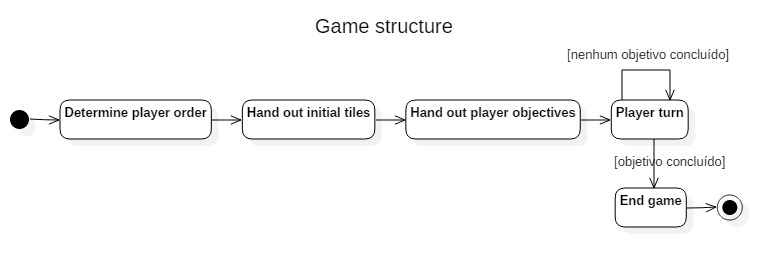
\includegraphics[width=130mm, scale=0.6]{images/Model__Game__Game_1.jpg}
}
\caption{Representação em máquina de estados das etapas do jogo}
\legend{Fonte: Os Autores}
\label{fig:smGame}
\end{figure}

\begin{figure}
\centering {
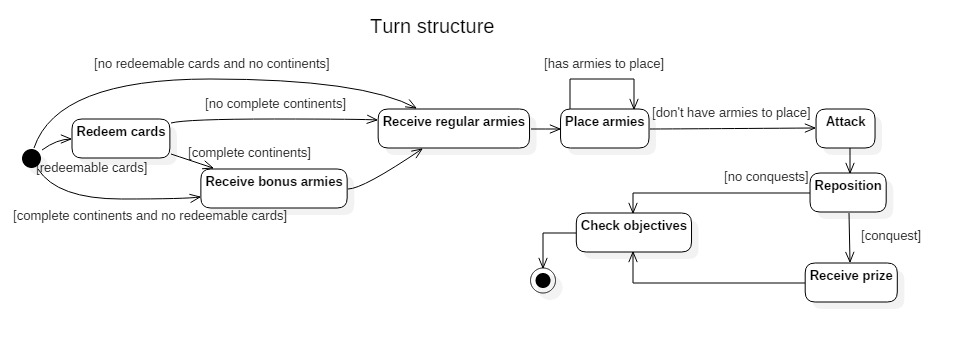
\includegraphics[width=130mm, scale=0.6]{images/Model__Turn__Turn_2.jpg}
}
\caption{Representação em máquina de estados das etapas do turno}
\legend{Fonte: Os Autores}
\label{fig:smTurn}
\end{figure}

O jogo de tabuleiro \textit{War} (\textit{Risk} na sua versão orignal) é um jogo de estratégia no qual cada jogador controla exércitos em uma missão de dominação mundial. A dinâmica do jogo consiste em expandir o seu domínio sobre o tabuleiro participando de combates contra os exércitos dos outros jogadores \cite{riskMan}.

Na etapa inicial do jogo, cada jogador escolhe para si, em turnos, um território desocupado do tabuleiro até que não existam mais territórios desocupados. Em cada um dos territórios escolhidos, o jogador coloca uma peça representando o seu exército de ocupaçao no território. Em seguida cada jogador recebe uma quantidade de exércitos definida de acordo com a quantidade de jogadores. Os jogadores novamente se revezam em turnos posicionando cada um desses exércitos em territórios sob o seu controle. Quando todos os exércitos são posicionados dessa forma, o jogo avança para a próxima etapa.

Na etapa seguinte, os jogadores se revezam em turnos para reforçar suas posições em territórios já ocupados e combater os exércitos dos territórios dos oponentes. Cada turno começa com o jogador ativo recebendo exércitos de acordo com a quantidade de territórios possuídos e os posicionando em seus territórios. Uma vez que todos os exércitos do turno tenham sido posicionados, o jogador pode escolher qualquer território seu que possui mais de um exército e declarar um ataque contra um território vizinho que seja controlado por um oponente. Em cada turno, o jogador pode escolher atacar quantas vezes quiser desde que possua territórios com mais de um exército.

No combate, o jogador atacante escolhe até 3 exércitos no território atacante e rola um dado de ataque para cada exército escolhido. O jogador defensor escolhe até 2 exércitos no território atacado e rola um dado de defesa para cada exército escolhido. A maior rolagem de ataque é então comparada com a maior rolagem de defesa e, caso seja maior, um exército do território atacado é removido do tabuleiro. Caso a rolagem de ataque seja igual ou menor que a rolagem de defesa, um exército do território atacante é removido. Esse procedimento se repete para as próximas maiores rolagens de ataque e defesa enquanto houverem dados para serem comparados. Ao final desse processo, se o território atacado acabar sem exércitos, o jogador atacante move os exércitos atacantes que restaram para esse território.

O sequênciamento dessas ações no jogo podem ser representadas por máquinas de estados e essa representação foi a que guiou o desenvolvimento da solução. A Figura \ref{fig:smGame} representa a sequência de etapas do jogo, a Figura \ref{fig:smTurn} representa a sequências de fases de um turno e a Figura \ref{fig:smAttack} representa as etapas de um combate.

\begin{figure}
\centering {
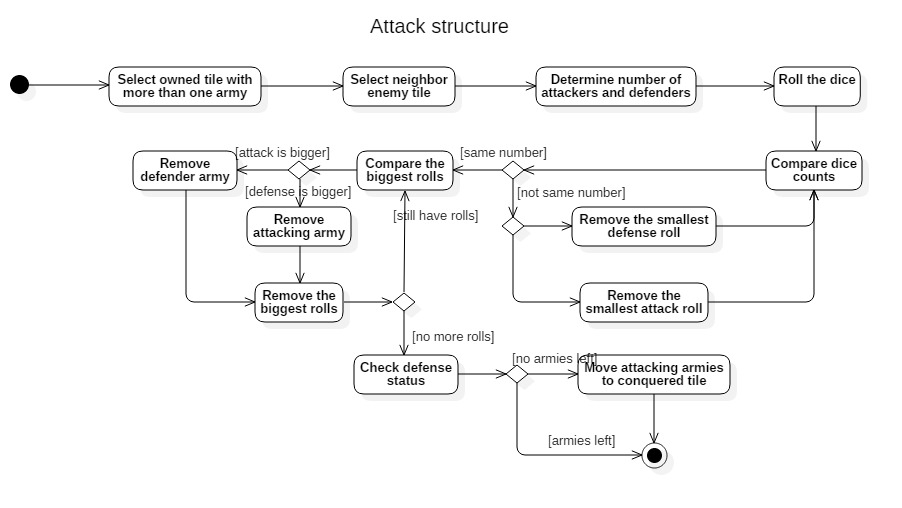
\includegraphics[width=130mm, scale=0.6]{images/Model__Attack__Attack_4.jpg}
}
\caption{Representação em máquina de estados das etapas do combate}
\legend{Fonte: Os Autores}
\label{fig:smAttack}
\end{figure}




%%%%%%%%%%%%%%%%%%%%%%%%%%%%%%%%%%%%%%%%%%%%%%%%%%%%%%%%%%%%%%%%%%%%%%%%%%%%%%%%%%%%%
% Capítulo 3
%
\chapter{Abordagem orientada a objetos}



\section{Classes}

As classes são a base da orientação a objetos. A figura 2.1 representa o diagrama de classes UML modelado para este projeto e utilizado como base para implementação do mesmo.
\begin{figure}[ht]
\centering {
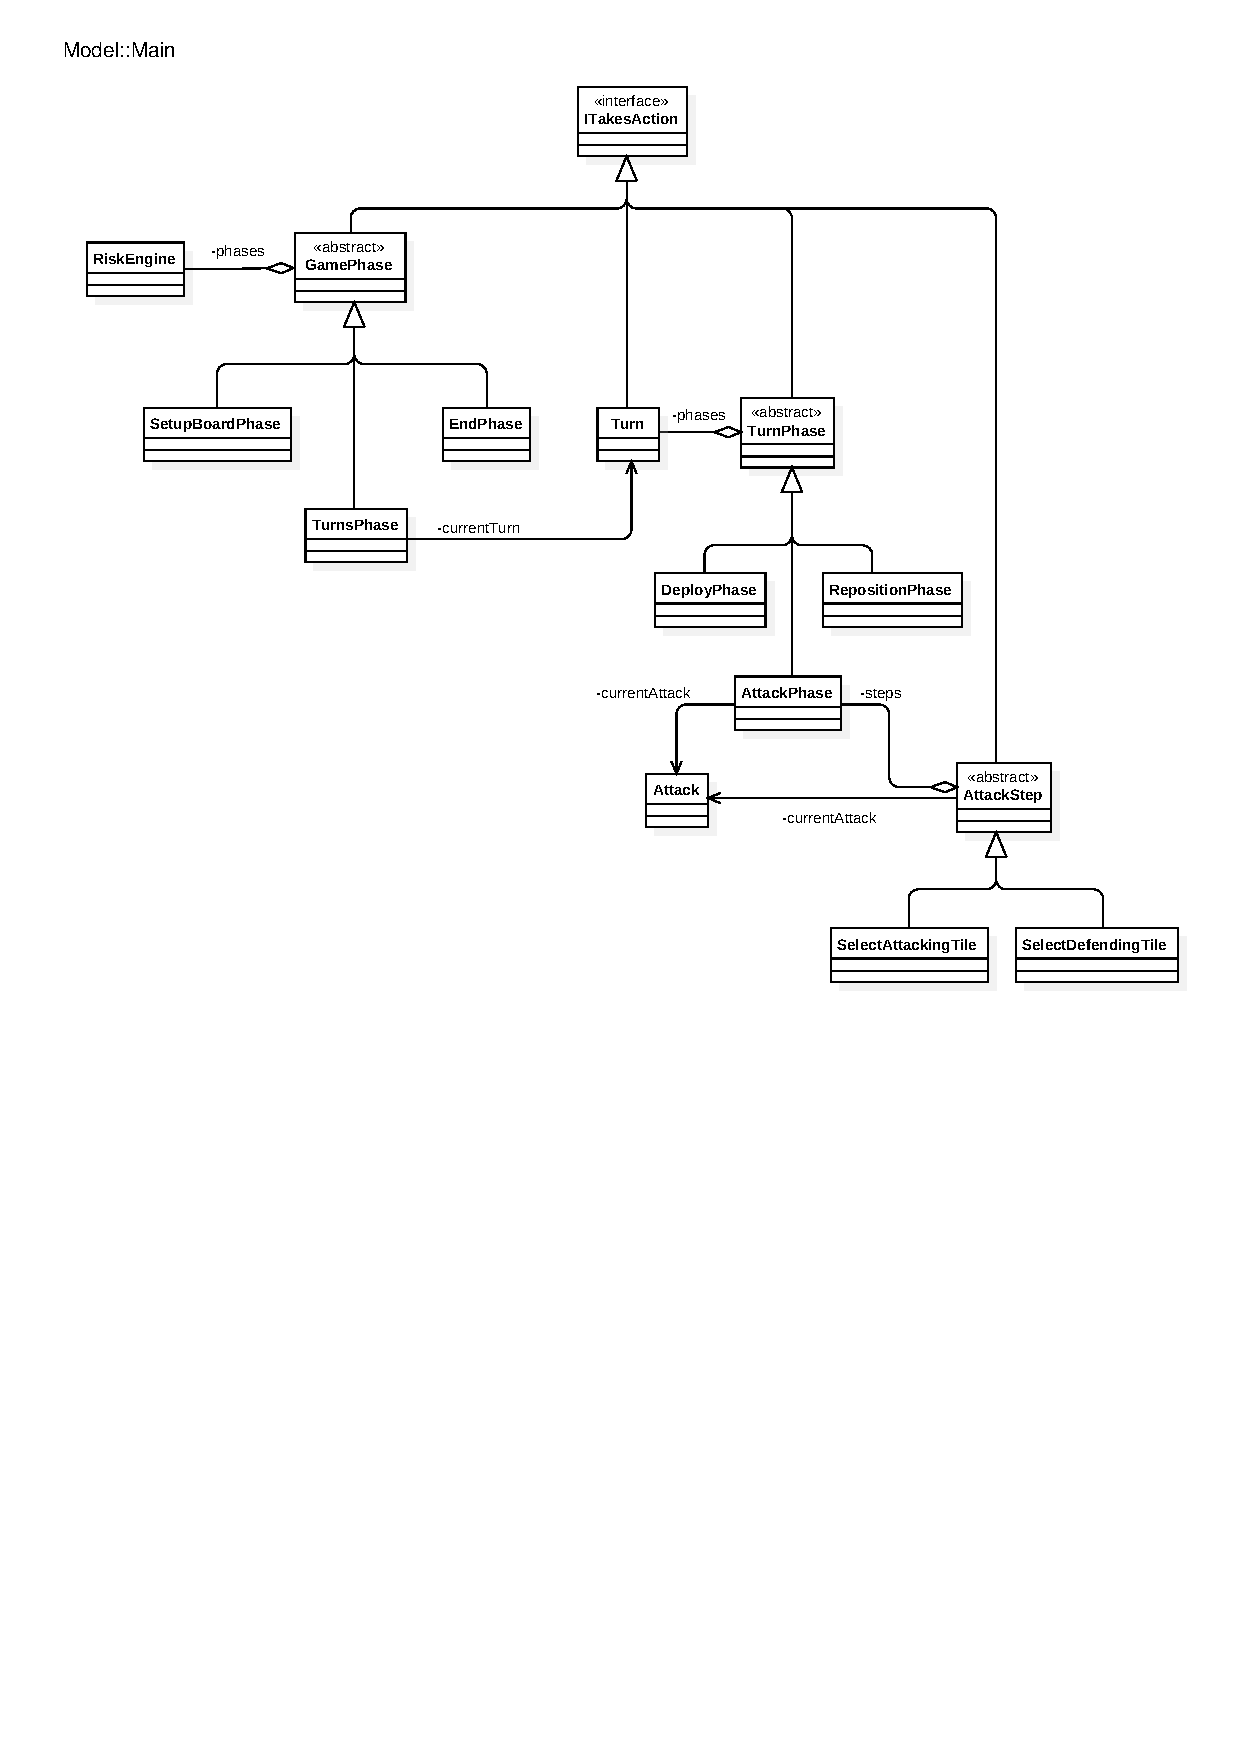
\includegraphics[width=130mm, scale=0.6]{uml/ClassDiagram.pdf}
}
%\lstinputlisting[firstline=37, lastline=45]{../src/classes/RiskEngine.ts}
%\lstinputlisting{../src/Interfaces/IRisk.ts}
\caption{Typescript class}
\label{fig:tsClass}
\end{figure}


\section{Encapsulamento}

O encapsulamento envolve a abstração dos métodos e atributos de determinada classe, tornando o software mais flexível à mudanças, já que cada funcionalidade deve ser implementada isolada das demais. Nesta implementação, 

\section{Construtores}

Blabla sobre construtores

\section{Destrutores}

Blabla sobre destrutores

\section{Namespaces}

Blabla sobre namespaces

\section{Herança}

Blabla sobre herança

\section{Polimorfismo por inclusão}

Blabla sobre polimorfirmo por inclusão

\section{Polimorfismo paramétrico}

Blabla sobre polimorfirmo paramétrico

\section{Polimorfismo por sobrecarga}

Blabla sobre polimorfirmo por sobrecarga

\section{Delegates}

Blabla sobre delegates

%%%%%%%%%%%%%%%%%%%%%%%%%%%%%%%%%%%%%%%%%%%%%%%%%%%%%%%%%%%%%%%%%%%%%%%%%%%%%%%%%%%%%
% Capítulo 3
%
\chapter{Abordagem funcional}


%%%%%%%%%%%%%%%%%%%%%%%%%%%%%%%%%%%%%%%%%%%%%%%%%%%%%%%%%%%%%%%%%%%%%%%%%%%%%%%%%%%%%
% Conclusões
%
\chapter{Conclusão}

\section{Abordagem orientada a objetos}

Descrever as facilidades e dificuldades encontradas, benefícios, problemas e limitações da linguagem estudada.


%%%%%%%%%%%%%%%%%%%%%%%%%%%%%%%%%%%%%%%%%%%%%%%%%%%%%%%%%%%%%%%%%%%%%%%%%%%%%%%%%%%
% Referências 
%%%%%%%%%%%%%%%%%%%%%%%%%%%%%%%%%%%%%%%%%%%%%%%%%%%%%%%%%%%%%%%%%%%%%%%%%%%%%%%%%%%
%

%\bibliographystyle{abnt}

\bibliographystyle{abntex2-alf}


\bibliography{biblio} % arquivo que contém as referências (no formato bib). Colocar as suas lá (se tiver dúvida sobre como adicionar novas referências, usar o software JabRef ou Medley)




\end{document}
